\documentclass[11pt,a4paper]{article}

\usepackage[margin=1in]{geometry}
\usepackage{amsmath}
\usepackage{graphicx}
\usepackage{booktabs}
\usepackage{hyperref}
\usepackage{caption}
\usepackage{subcaption}
\usepackage{float}
\usepackage{parskip}
\usepackage{xcolor}

\hypersetup{colorlinks=true, linkcolor=blue, citecolor=blue, urlcolor=blue}

\title{\textbf{Predicting Review Usefulness on Yelp:\\
A Multi-Class Classification Study}}
\author{Brian Ko}
\date{\today}

\begin{document}

\maketitle
\tableofcontents
\newpage

% ================================================================
\section{Introduction}
% ================================================================

Online review platforms such as Yelp play a central role in consumer
decision-making. Among the millions of reviews posted daily, not all
are equally informative. Yelp allows users to vote on whether a review
is ``useful'', producing a count of usefulness votes per review. This
signal reveals the perceived quality of a review from the community's
perspective, yet predicting it automatically remains a challenging
natural language and social computing problem.

Automatically identifying which reviews are likely to be perceived as
useful has practical value: it can help surfaces high-quality content
to readers, guide recommendation systems, and assist content moderation.
Prior work has largely framed this as binary classification (useful
vs.\ not useful), which collapses the nuanced spectrum of community
engagement into a single threshold.

In this work, we formulate review usefulness prediction as a
\textbf{four-class classification} problem. We define four ordinal
classes based on the raw useful vote count and evaluate two
complementary models: (1) \textbf{XGBoost}, a gradient-boosted tree
model operating on structured tabular features, and (2) a
\textbf{Multi-Layer Perceptron (MLP)}, which jointly leverages both
tabular features and TF-IDF text representations. We compare their
performance on the Yelp Open Dataset and analyze feature importance to
understand what drives usefulness.

% ================================================================
\section{Method}
% ================================================================

\subsection{Label Definition}

We define four ordinal usefulness classes based on the number of useful
votes $u$ a review has received:

\begin{table}[H]
\centering
\caption{Four-class label definition.}
\begin{tabular}{cll}
\toprule
\textbf{Class} & \textbf{Label} & \textbf{Condition} \\
\midrule
0 & None   & $u = 0$ \\
1 & Low    & $u = 1$ \\
2 & Medium & $2 \leq u \leq 3$ \\
3 & High   & $u \geq 4$ \\
\bottomrule
\end{tabular}
\end{table}

\subsection{Feature Engineering}

We derive two types of features from the Yelp dataset:

\paragraph{Tabular features (25 dimensions).}
These include review-level signals (star rating, text length, word count,
punctuation counts, uppercase ratio, review date), business-level signals
(business stars, review count, check-in count, category count, open
status), and user-level signals (review count, average stars, years on
Yelp, fans, aggregate useful/funny/cool votes, elite years, friend count).
All continuous features are standardized using \texttt{StandardScaler}
fit on the training set only.

\paragraph{TF-IDF features (5000 dimensions).}
We apply TF-IDF vectorization with unigrams and bigrams
(\texttt{ngram\_range=(1,2)}), sublinear TF scaling, and a minimum
document frequency of 5, retaining the top 5{,}000 terms by TF-IDF score.
The vectorizer is fit on the training set only.

\subsection{Models}

\paragraph{XGBoost.}
We train an XGBoost classifier with the \texttt{multi:softprob} objective
using both tabular and TF-IDF features concatenated as a sparse matrix.
Key hyperparameters: 500 estimators, max depth 6, learning rate 0.05,
subsample ratio 0.8, column subsample ratio 0.8. Early stopping
(patience = 20) is applied on the validation set using multi-class
log-loss (\texttt{mlogloss}).

\paragraph{MLP.}
We train a feed-forward neural network on the concatenated tabular +
TF-IDF input (5{,}025 dimensions). The architecture is:
\[
\text{Linear}(5025 \to 512) \to \text{BN} \to \text{ReLU} \to \text{Dropout}(0.3)
\to \text{Linear}(512 \to 256) \to \text{BN} \to \text{ReLU} \to \text{Dropout}(0.3)
\to \text{Linear}(256 \to 64) \to \text{ReLU}
\to \text{Linear}(64 \to 4)
\]
Training uses Adam optimizer (lr $= 10^{-3}$, weight decay $= 10^{-4}$),
cross-entropy loss, a batch size of 2{,}048, and early stopping with
patience 5 on validation loss. A \texttt{ReduceLROnPlateau} scheduler
(factor 0.5, patience 2) is applied.

% ================================================================
\section{Experiments}
% ================================================================

\subsection{Dataset}

We use the \textbf{Yelp Open Dataset}, which contains approximately
7 million reviews across businesses in multiple US cities. After joining
reviews with business, user, and check-in tables, we construct a balanced
sample by drawing 578{,}664 reviews from each of the four usefulness
classes, yielding a total of \textbf{2{,}314{,}656 rows}.

\begin{table}[H]
\centering
\caption{Balanced dataset statistics.}
\begin{tabular}{lr}
\toprule
\textbf{Property} & \textbf{Value} \\
\midrule
Total reviews (balanced)     & 2{,}314{,}656 \\
Reviews per class            & 578{,}664 \\
Number of classes            & 4 \\
Tabular features             & 25 \\
TF-IDF features              & 5{,}000 \\
Total input dimensions (MLP) & 5{,}025 \\
\bottomrule
\end{tabular}
\end{table}

\subsection{Data Splits}

The balanced dataset is split into train, validation, and test sets
using stratified sampling to preserve class proportions:

\begin{table}[H]
\centering
\caption{Train/validation/test split sizes.}
\begin{tabular}{lr}
\toprule
\textbf{Split} & \textbf{Size} \\
\midrule
Train      & $\sim$1{,}660{,}000 \\
Validation & $\sim$290{,}000 \\
Test       & $\sim$347{,}000 \\
\bottomrule
\end{tabular}
\end{table}

\subsection{Evaluation Metrics}

We report accuracy, macro-averaged precision, recall, and F1-score,
weighted F1-score, and macro-averaged one-vs-rest (OvR) ROC-AUC. Because
the balanced dataset has equal class prior, macro and weighted averages
coincide.

% ================================================================
\section{Results}
% ================================================================

\subsection{Main Performance (Table 1)}

Table~\ref{tab:main} reports test-set performance for both models.
The MLP outperforms XGBoost on all metrics, achieving an accuracy of
54.0\% vs.\ 53.2\% and a ROC-AUC of 0.807 vs.\ 0.801. Both models
substantially exceed the random baseline of 25\% (four equal classes),
demonstrating that the features contain meaningful signal. The modest
absolute accuracy reflects the inherent difficulty of distinguishing
adjacent ordinal classes (e.g., one vs.\ two useful votes).

\begin{table}[H]
\centering
\caption{Main performance comparison on the test set.}
\label{tab:main}
\begin{tabular}{lcc}
\toprule
\textbf{Metric}            & \textbf{XGBoost} & \textbf{MLP} \\
\midrule
Accuracy                   & 0.5315           & 0.5400 \\
Precision (macro)          & 0.5275           & 0.5378 \\
Recall (macro)             & 0.5315           & 0.5400 \\
F1 (macro)                 & 0.5282           & 0.5384 \\
F1 (weighted)              & 0.5282           & 0.5384 \\
ROC-AUC (OvR macro)        & 0.8005           & 0.8067 \\
\bottomrule
\end{tabular}
\end{table}

\subsection{MLP Training Curves (Figure 1)}

Figure~\ref{fig:training} shows the MLP training and validation loss
alongside the validation ROC-AUC across 19 epochs. The model converges
steadily, reaching a best validation ROC-AUC of \textbf{0.8068} before
early stopping is triggered. The small gap between training loss
(0.954) and validation loss (0.984) indicates mild overfitting, which
is controlled by dropout and weight decay.

\begin{figure}[H]
\centering
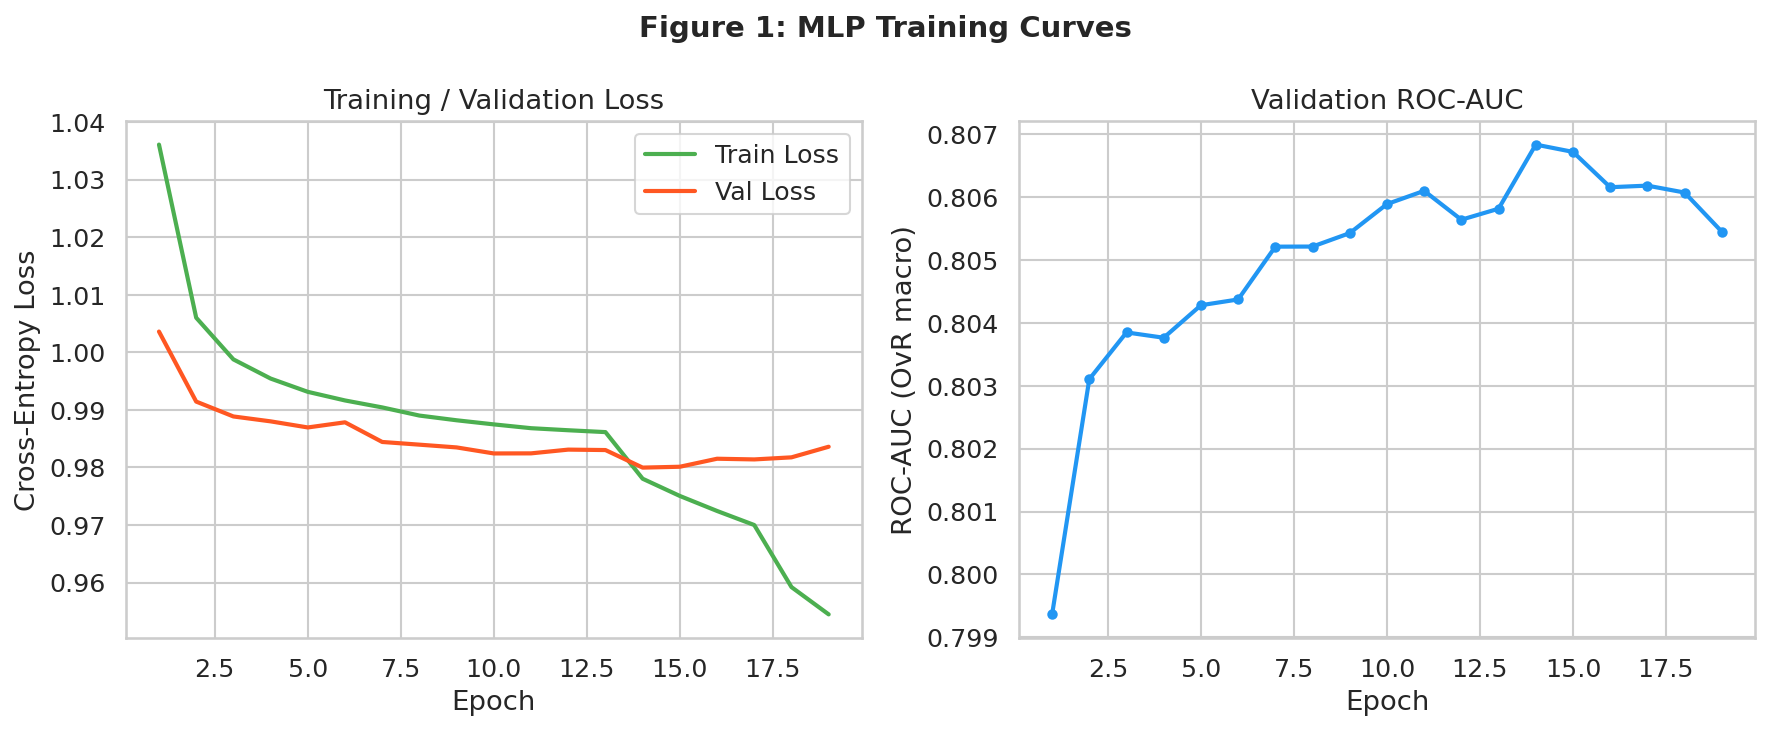
\includegraphics[width=\linewidth]{figure1_mlp_training_loss.png}
\caption{Figure 1: MLP training and validation loss (left) and
         validation ROC-AUC (right) over training epochs.}
\label{fig:training}
\end{figure}

\subsection{Feature Importance (Figure 2)}

Figure~\ref{fig:importance} shows the top-15 features for both models.

For \textbf{XGBoost} (gain importance), the most informative features
are \texttt{user\_useful} (0.217), \texttt{user\_cool} (0.151), and
\texttt{review\_text\_len} (0.135). This suggests that a user's
historical reputation on Yelp is a strong proxy for whether their
reviews will be perceived as useful. Review length is the strongest
purely content-based signal.

For the \textbf{MLP} (permutation importance, OvR ROC-AUC drop),
\texttt{user\_useful} (0.299) is again dominant, followed by
\texttt{user\_review\_count} (0.135) and \texttt{user\_cool} (0.061).
The larger importance of \texttt{user\_useful} in the MLP compared to
XGBoost suggests that, even alongside 5{,}000 TF-IDF text features,
user reputation remains the most decisive single tabular feature.

\begin{figure}[H]
\centering
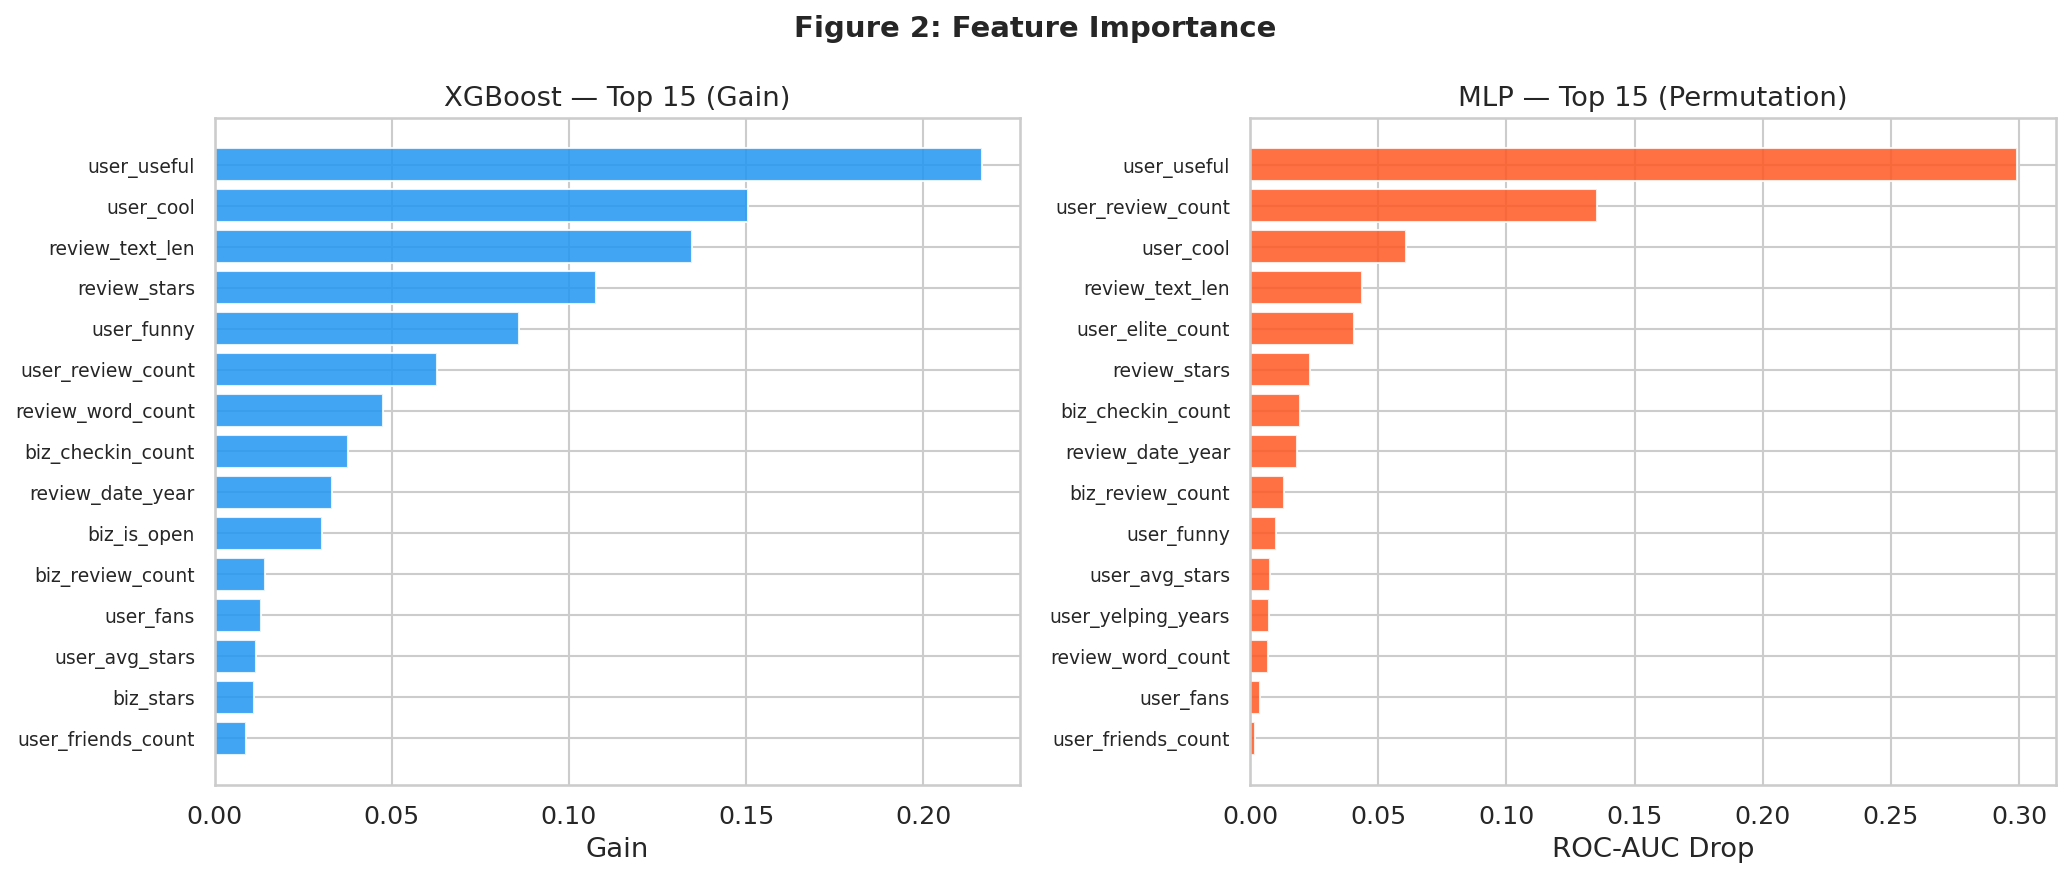
\includegraphics[width=\linewidth]{figure2_feature_importance.png}
\caption{Figure 2: Top-15 feature importances. Left: XGBoost gain
         importance. Right: MLP permutation importance (OvR ROC-AUC drop).}
\label{fig:importance}
\end{figure}

% ================================================================
\section{Conclusion}
% ================================================================

We presented a four-class formulation of Yelp review usefulness
prediction and evaluated two models — XGBoost and MLP — on a balanced
sample of over 2.3 million reviews. Both models substantially outperform
random chance (25\%), with the MLP achieving the best performance
(accuracy 54.0\%, ROC-AUC 0.807) by jointly exploiting tabular and
text features.

Feature importance analysis reveals that \textbf{user reputation features}
— in particular the aggregate useful votes a user has accumulated
historically — are the most predictive signals in both models, outweighing
purely content-based features such as review length or text vocabulary.
This raises an important consideration: user reputation features may
constitute a proxy for the target label rather than an independent
predictor of review quality. Future work could ablate these features to
isolate the contribution of review content alone.

The modest accuracy ($\sim$54\%) reflects the difficulty of the task.
Adjacent ordinal classes (e.g., 1 vs.\ 2 useful votes) are largely
indistinguishable from content alone, as vote counts depend partly on
random exposure effects. Directions for future improvement include
using pre-trained language models (e.g., BERT) for richer text
representations, incorporating social graph features, and formulating
the task as ordinal regression to better exploit the natural ordering
of the classes.

\end{document}
